\section{Coinciding Vertices}
The \texttt{coincidingVertices} function is an essential component in mesh processing algorithms, designed to identify and handle vertices with the same coordinates. This functionality becomes crucial in scenarios where mesh data contains overlapping vertices due to precision limitations or data noise.\\

An example for the usage of \texttt{coincidingVertices} can be found in \autoref{subsec:connected_Components}. While we can see the four components of the teapot neatly displayed in \autoref{fig:teapotcomps} this is after identifying similar vertices with each other. Just taking the original data and looking at the connected components results in a surprising amount of components.

\begin{lstlisting}[language=Python, caption={Connected components with and without \texttt{coincidingVertices}}, label={lst:coincidingVertices}]
from maniflow.mesh import Mesh
from maniflow.mesh.obj import OBJFile
from maniflow.mesh.utils import connectedComponents, coincidingVertices

teapot = OBJFile.read("examples/teapot.obj")  # reading the mesh from memory

print(f"Without coinciding the vertices there are {len(connectedComponents(teapot))} components.")

coincidingVertices(teapot)  # identifying and collapsing coinciding vertices
print(f"After coinciding the vertices there are {len(connectedComponents(teapot))} components.")
\end{lstlisting}

\begin{lstlisting}[escapeinside={<@}{@>}]
Without coinciding the vertices there are 19 components.
After coinciding the vertices there are 4 components.
\end{lstlisting}

What happened here is that the four intuitively expected components had been designed as quarters and then assembled. To the eye it does not make a difference but for the code it does.

Looking at some of the $19$ components we see that the teapot seems to have been created by having parts of a repeating object, say the floor of the teapot where there are four quarters of, being moved and turned to fit together. For example, by running \autoref{lst:teapot_four_components} without \texttt{coincidingVertices} in line 6 we end up getting said $19$ components as .obj-files. Then running

\begin{lstlisting}[language=Python, caption={Visualizing the parts of the bottom of the teapot}, label={lst:teapot_btm_parts}]
from maniflow.mesh.parameterized import *
from maniflow.mesh.obj import OBJFile
from maniflow.render import SVGPainterRenderer
from maniflow.render.scene import *

# 4 times as we have four parts of the bottom of the teapot
for i in range(4):
    teapot_btm = OBJFile.read(f"teapot{16+i}.obj")
    # Invert orientation for colour visibility
    for j in range(teapot_btm.f):
        teapot_btm.faces[j].vertices = teapot_btm.faces[j].vertices[::-1]
    # Setting up renderer
    teapot_btm.setStyle('red')
    camera = Camera(position(10,-20,5), target=(0, -0.7, 0))
    scene = Scene(camer=camera, width=400, height=400, light=np.array([10, -1.5, 50]
    renderer = SVGPainterRenderer(scene)
    # Take image and save it
    image = renderer.render(teapot_btm)
    image.save_svg(f"teapot_part{i+1}_render.svg")
\end{lstlisting}

gets us the four components that form the bottom of the teapot in \autoref{fig:teapot_parts}:

\begin{figure}[H]%
\scalebox{.75}{
\centering
\subfloat[First part]{\includesvg[width=0.35\textwidth]{img/teapot_part2_render.svg}}\qquad
\subfloat[Second part]{\includesvg[width=0.25\textwidth]{img/teapot_part1_render.svg}}\qquad
\subfloat[Third part]{\includesvg[width=0.25\textwidth]{img/teapot_part3_render.svg}}\qquad
\subfloat[Forth part]{\includesvg[width=0.35\textwidth]{img/teapot_part4_render.svg}}\qquad}
\caption{The quarters of the bottom of the teapot.}
\label{fig:teapot_parts}
\end{figure}

Similarly, when we take a look at the moebius strip generated from a grid, we note that while the ends have the same points they still are not glued together. Again, to the eye there is no difference but topologically the moebius strip created from the grid is then just a plain with Euler Characteristic $1$. Yet, it is well-known that an actual moebius strip has an Euler Characteristic of $0$. Using \texttt{coincidingVertices} we can glue those loose ends together to get:

\begin{lstlisting}[language=Python, caption={Euler Characteristic of the moebius strip with and without \texttt{coincidingVertices}}, label={lst:coincidingVertice_eulers}]
import numpy as np
from maniflow.mesh.parameterized import *

@VertexFunction
def moebius(vertex):
    x = vertex[0]
    y = vertex[1]
    x0 = np.cos(x) * (1 + (y / 2) * np.cos(x / 2))
    x1 = np.sin(x) * (1 + (y / 2) * np.cos(x / 2))
    x2 = (y / 2) * np.sin(x / 2)
    return np.array([x0, x1, x2])

u = Grid((0, 2 * np.pi), (-1, 1), 30, 10)  # create a high resolution grid
moebiusMesh = moebius(u)

print(f"Euler Characteristic before coincidingVertices: {eulerCharacteristic(moebiusMesh)}")
coincidingVertices(moebiusMesh)
print(f"Euler Characteristic after coincidingVertices: {eulerCharacteristic(moebiusMesh)}")
\end{lstlisting}

\begin{lstlisting}[escapeinside={<@}{@>}]
Euler Characteristic before coincidingVertices: 1
Euler Characteristic after coincidingVertices: 0
\end{lstlisting}

\subsection{The Upper Triangular Approach}
The old version of \texttt{coincidingVertices} utilizes an approach with a time complexity of $O(n^2)$, where $n$ represents the number of vertices in the mesh. This stems from iterating twice through all or at least a linearly decreased subset of the vertex data. While being naive in its concept there are a few tweaks that improve the algorithm, more than halving its runtime. That of course is not as good as it sounds given that we have a quadratic runtime nature.

It starts by initializing empty data structures, iterates through each vertex to detect coinciding vertices, merges them into a single vertex, and updates the mesh accordingly. To reduce computational power needed this naive approach is improved by the simple fact that if $a == b$ then also $b == a$, so this halves the amount of iteration steps in a double for-loop leading to these computations. This leaves us with an upper triangular form where we only have to check the following indices but not the previous as those where checked before. E.g. when checking whether the third vertex can be identified with another vertex we can start at the fourth vertex since, say, the check against the second vertex already happened when we previously check for identities with the second vertex. The resulting checks can be visualized in a matrix looking similar to this
\begin{center}
\begin{tabular}{|*{7}{c|}}
                               \hline
    & 1 & 2 & 3 & 4 & 5 & n \\ \hline
  1 &   & X & X & \checkmark & X & X \\ \hline
  2 &   &   & X & - & X & X \\ \hline
  3 &   &   &   & - & X & X \\ \hline
  4 &   &   &   &   & - & - \\ \hline
  5 &   &   &   &   &   & X \\ \hline
  n &   &   &   &   &   &   \\ \hline
\end{tabular}
\end{center}

where the 'X' implies a comparison to be done and the '\checkmark' denotes, in this case, that the first vertex and the fourth vertex are the same point with regard to our tolerance. This results in canceling all checks for (row) and against (column) the fourth vertex as this check has been done for the identical first vertex already, indicated by '-'. Because of this canceling we get a best case scenario of $O(n)$ that is if all vertex are identified to be the same point. After one iteration through all of them we have identified them all with the first vertex resulting in not going through their rows and columns. This leaves only the first $n$ checks.
\begin{center}
\begin{tabular}{|*{7}{c|}}
                               \hline
    & 1 & 2 & 3 & 4 & 5 & n \\ \hline
  1 &   & \checkmark & \checkmark & \checkmark & \checkmark & \checkmark \\ \hline
  2 &   &   & - & - & - & - \\ \hline
  3 &   &   &   & - & - & - \\ \hline
  4 &   &   &   &   & - & - \\ \hline
  5 &   &   &   &   &   & - \\ \hline
  n &   &   &   &   &   &   \\ \hline
\end{tabular}
\end{center}

\subsubsection{Bubblesort by accident}
Without realizing at the time of first implementation the upper triangular approach is equivalent to the Bubblesort sorting algorithm. As a reminder, Bubblesort also first iterates through all elements. At the end of the iteration one of the elements is at its proper place. Afterwards, it repeats with the next iteration but this time it can leave out checking said element. Bubblesort functions in the following way:\\
\begin{algorithm}[H]
    \SetAlgoLined
    \SetKwInOut{Input}{Input}
    \SetKwInOut{Output}{Output}

    \Input{List of sortable elements}
    \Output{Sorted List}
    \caption{Bubblesort}
    \label{alg:bubblesort}
    \KwData{List}
    \For{i := 1 to n - 1}{
        Set swapped flag to False\;
        \For{j :=1 to n - i}{
            \If{j-th element is smaller than (j-1)-th element}{
                Swap the two elements\;
                Set swapped flag to True\;
            }
        }
        \If{swapped flag is set to False}{
            Stop\;
        }
    }
\end{algorithm}

This is essentially the algorithm used for the upper triangular approach with the only difference being the direction of the inner loop, i.e. for the $i$-th row it starts from the at $i+1$ and ends at the end $n$ for the upper triangular but Bubblesort always starts at the beginning and ends at $n-i$.\\
The advantage we get now is that the runtime performance of Bubblesort is well known. Having the same structure this means that our upper triangular approach we ca not only confirm the performance mentioned above, that is $O(n)$ in the best case and $O(n^2)$ in the worst case, but also get the average case from Bubblesort, which is $O(n^2)$ as well.

\subsection{Time to sort - Using Timsort to speed things up}
The updated version of \texttt{coincidingVertices} employs a more efficient approach compared to the old version. It starts by creating an empty list \texttt{extVertList} and copies the mesh's faces into \texttt{faceList}. It then iterates through each face and its vertices, adding the $j$-th vertex in the $i$-th face along with the information on $i$ and $j$ to \texttt{extVertList}. Next, it sorts \texttt{extVertList} by the first element (the vertex coordinates) using Python's Timsort algorithm, resulting in a stable sorting with an average time complexity of $O(n\log n)$. Overall, timsort is linear with $O(n)$ in the best case as it is an adaptive sorting algorithm, and capped in the worst case at $O(n\log n)$.

The function then initializes an empty list \texttt{vertList} and iterates through all entries of \texttt{extVertList}. For each entry \texttt{v}, it checks if \texttt{vertList} is empty or if the vertex is not close to the previous one. If so, it adds the vertex to \texttt{vertList}. Additionally, it updates the vertices in \texttt{faceList} based on the indices in \texttt{vertList}, ensuring that vertices with the same coordinates are identified and glued together.

\begin{algorithm}[H]
    \SetAlgoLined
    \SetKwInOut{Input}{Input}
    \SetKwInOut{Output}{Output}

    \Input{Mesh}
    \Output{Mesh with identified vertices}
    \caption{coincidingVertices Timsort}
    \label{alg:coincidingVertices_timsort}
    \KwData{mesh}
    Initialize list 'extVertList'\;
    Create work copy 'faceList' of the faces of the mesh\;
    \For{every face in 'faceList'}{
        \For{every vertex in the face}{
            Add [coordinate of vertex, index of face, index of vertex] to 'extVertList'\;
        }
    }
    Sort 'extVertList' by coordinates, starting with the first\;
    Initialize list 'vertList'\;
    \For{every entry 'v' in 'extVertList'}{
        \If{either 'vertList' is empty or the latest entry of 'vertList' is not close to 'v'}{
            Add 'v' to 'vertList'\;
        }
        Update the vertex in the face referenced in 'v'\;
    }
    Copy the values of 'faceList' into the initial mesh\;
\end{algorithm}

Note that the definition of closeness is not the standard metric but whether the vertices can be fitted into a box of size $2\textit{atol} \times 2\textit{atol} \times 2\textit{atol}$. While not as intuitive as a simple distance between the points in the three dimensional, this allows us to use the a sorting algorithm since the vertices have to be within \texttt{atol} on \textit{all} three coordinate axis. This means we can start looking at the first coordinate, compare that and, if it is within tolerance, we can continue with the second and third if needed. Hence, we can sort the first coordinates (if equal then go by the second, etc.). This approach can be used, as we did, to implement a fast algorithm that only needs to check the previous vertex for equality since it is the closest yet tested vertex, at least on the first coordinate. And since we are checking not the Euclidean distance between points but have this box approach all of the coordinates have to be contained. Thus, we can stop if the first coordinate is not close. If it is, we check for the second coordinate. As these are sorted as well, the latest entry to \texttt{vertList} has to be the closest to the currently checked vector in the second coordinate as well, given closeness in the first. This can be applied to the third coordinate as well.

By using not only the fast sorting of timsort but also being able to just check against a single different point (so comparing up to three different floats) this algorithm is very fast and efficient. Since we just iterate once through the faces and their three respective vertices ($3n$ operations), sorting with on average (and even in the worst case) $O(n\log n)$ and then iterate again only once though the list \texttt{extVertList} of length $n$, we end up with $O(3n)+O(n\log n)+O(n)=O(n\log n)$ as overall runtime.

\subsection{Time comparison}
A direct comparison can be drawn by using the \texttt{timeit}-package in Python. Since \texttt{coincidingVertices} normally overwrites the mesh given in the parameter we need to make adjustments to the functions for example introducing a variable called 'dummy' that is written into instead of the original mesh. It is only used for this writing of data and the timing method applied here.

The comparison will be drawn between the two implementations using the teapot OBJ-file already present. It consists of $3644$ vertices which both functions will bring down to $3241$. This is a decrease of about about 11.1\% or one in every nine vertices being identified with another vertex.

As the main load of the computation is on the naive double-looping (upper triangle) and the sorting algorithm we can expect the other calls in the functions such as list manipulations and calls to stored data to be insignificant with the difference in performance being $O(n^2)$ and $O(n\log n)$ on average for a relatively (to simpler shapes) large $n=3644$.

\begin{lstlisting}[language=Python, caption={Timing Comparison between Upper Triangular and Timesort Approach}, label={lst:timing_comparison}]
from timeit import default_timer as timer

teapot = OBJFile.read("examples/teapot.obj")

repetitions = 10    # coincidingVertices_old is SIGNIFICANTLY slower than the newer version, choose repetitions accordingly
time_a = 0
time_b = 0

# cumulated time for the upper triangular method
for i in range(repetitions):
    start = timer()
    coincidingVertices_old(teapot)
    end = timer()
    time_a = time_a + (end - start)

# cumulated time for the timsort method
for i in range(repetitions):
    start = timer()
    coincidingVertices_new(teapot)
    end = timer()
    time_b = time_b + (end - start)

print(f"Upper Triangle Approach execution time avg.: {time_a/repetitions} seconds")
print(f"Sorting Algorithm Approach execution time avg.: {time_b/repetitions} seconds")
\end{lstlisting}

The code outputs the following result
\begin{lstlisting}[escapeinside={<@}{@>}]
Upper Triangle Approach execution time avg.: 81.20345090379979 seconds
Sorting Algorithm Approach execution time avg.: 0.33098463589976745 seconds
\end{lstlisting}

This result is completely within expectation and still depicts nicely how even for a not extremely large $n=3644$ we already need about $245$ times longer with the upper triangular than with timesort. Since we are working with a non-small $n$ the quadratic nature of the upper triangular approach weights heavy on the runtime to the point that using for the renderer the upper triangular approach is simply not feasible.

\subsection{Further thoughts}
With this speedy approach come limitations, though. The algorithm does not care for relative closeness, all it looks at is \textit{whether} it is within \texttt{atol} but not \textit{how} close the vertices are when within this tolerance. This can lead to cases where for three points $[a, b, c]$ with $a$ and $b$ being close (as in within the \texttt{atol}-box) and $b$ and $c$ being close, but not $a$ and $c$.

The algorithm starts from $a$ and checks against $b$. They are close so it identifies $a$ and $b$ with coordinates of $a$. But then $a$ and $c$ are not close so they are not the same (w.r.t. the program) even though $b$ and $c$ might have been closer to each other than $a$ and $b$, see \autoref{fig:coinciding_vertices_a_start}. We hence can have non-optimal identifications for vertices which, again, is a trade-off that is made for increased computational efficiency.\\

\begin{figure}[t]
    \centering
    \subfloat[Identifying $b$ with $a$ as we start with $a$]{
        \centering
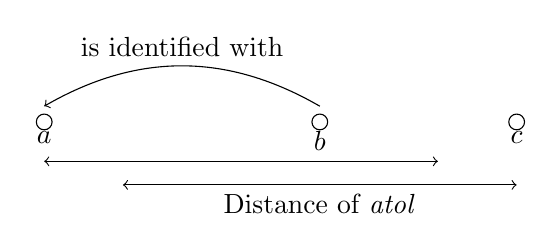
\begin{tikzpicture}
    % Define points a, b, and c
    \coordinate (a) at (0,0);
    \coordinate (b) at (3.5,0);
    \coordinate (c) at (6,0);

    % Draw circles around points a, b, and c
    \draw (a) circle [radius=0.1] node[below] {$a$};
    \draw (b) circle [radius=0.1] node[below] {$b$};
    \draw (c) circle [radius=0.1] node[below] {$c$};

    % Draw distance indicator
    \draw[<->] ([yshift=-0.5cm]a) -- node[below] {} ([xshift=-1cm,yshift=-0.5cm]c);
    \draw[<->] ([xshift=1cm,yshift=-0.8cm]a) -- node[below] {Distance of \textit{atol}} ([yshift=-0.8cm]c);

    % Draw curved arrow from b to a
    \draw[->, bend right] ([yshift=0.2cm]b) to node[above] {is identified with} ([yshift=0.2cm]a);
\end{tikzpicture}
}
\hfill
    \subfloat[$a$ and $c$ are not close enough for identification]{
    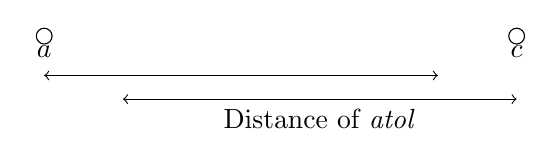
\begin{tikzpicture}
    % Define points a, b, and c
    \coordinate (a) at (0,0);
    \coordinate (c) at (6,0);

    % Draw circles around points a, b, and c
    \draw (a) circle [radius=0.1] node[below] {$a$};
    \draw (c) circle [radius=0.1] node[below] {$c$};

    % Draw distance indicator
    \draw[<->] ([yshift=-0.5cm]a) -- node[below] {} ([xshift=-1cm,yshift=-0.5cm]c);
    \draw[<->] ([xshift=1cm,yshift=-0.8cm]a) -- node[below] {Distance of \textit{atol}} ([yshift=-0.8cm]c);
\end{tikzpicture}
}
    \caption{Coinciding the vertices $a,b,c$ when starting with $a$}
    \label{fig:coinciding_vertices_a_start}
\end{figure}
%
\begin{figure}[t]
    \centering
    \subfloat[Identifying $a$ with $b$]{
        \centering
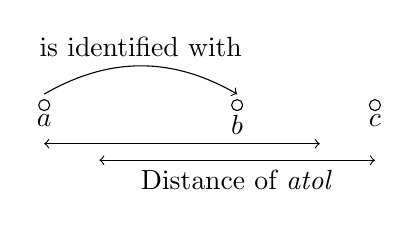
\begin{tikzpicture}[scale=0.7]
    % Define points a, b, and c
    \coordinate (a) at (0,0);
    \coordinate (b) at (3.5,0);
    \coordinate (c) at (6,0);

    % Draw circles around points a, b, and c
    \draw (a) circle [radius=0.1] node[below] {$a$};
    \draw (b) circle [radius=0.1] node[below] {$b$};
    \draw (c) circle [radius=0.1] node[below] {$c$};

    % Draw distance indicator
    \draw[<->] ([yshift=-0.7cm]a) -- node[below] {} ([xshift=-1cm,yshift=-0.7cm]c);
    \draw[<->] ([xshift=1cm,yshift=-1cm]a) -- node[below] {Distance of \textit{atol}} ([yshift=-1cm]c);

    % Draw curved arrow from b to a
    \draw[<-, bend right] ([yshift=0.2cm]b) to node[above] {is identified with} ([yshift=0.2cm]a);
\end{tikzpicture}
}
\hfill
    \subfloat[Identifying $c$ with $b$]{
    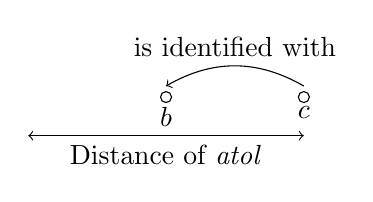
\begin{tikzpicture}[scale=0.7]
    % Define points a, b, and c
    \coordinate (a) at (0,0);
    \coordinate (b) at (3.5,0);
    \coordinate (c) at (6,0);

    % Draw circles around points a, b, and c
    \draw (b) circle [radius=0.1] node[below] {$b$};
    \draw (c) circle [radius=0.1] node[below] {$c$};

    % Draw distance indicator
    \draw[<->] ([xshift=1cm,yshift=-0.7cm]a) -- node[below] {Distance of \textit{atol}} ([yshift=-0.7cm]c);
    \draw[->, bend right] ([yshift=0.2cm]c) to node[above] {is identified with} ([yshift=0.2cm]b);
\end{tikzpicture}
}
\hfill
\subfloat[Only $b$ left, nothing to do]{
        \centering
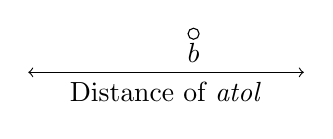
\begin{tikzpicture}[scale=0.7]
    % Define points a, b, and c
    \coordinate (a) at (0,0);
    \coordinate (b) at (3.5,0);
    \coordinate (c) at (6,0);

    % Draw circles around points a, b, and c
    \draw (b) circle [radius=0.1] node[below] {$b$};

    % Draw distance indicator
    \draw[<->] ([xshift=0.5cm,yshift=-0.7cm]a) -- node[below] {Distance of \textit{atol}} ([xshift=-0.5cm,yshift=-0.7cm]c);
\end{tikzpicture}
}
    \caption{Coinciding vertices this time starting with $b$}
    \label{fig:coinciding_vertices_b_start}
\end{figure}

Also note that the implemented function is iterating through the points in order that they are listed. Depending on the order in the list we can have different results visualized by comparing \autoref{fig:coinciding_vertices_a_start} and \autoref{fig:coinciding_vertices_b_start}. So if we were to start from vertex $b$ because it is mentioned before $a$ and $c$, this means that we check whether $b == a$ and not $a == b$, then $b$ and $a$ would be identified in the point $b$ and not $a$. As $b$ and $c$ are close as well, this would again be coincided in $b$ resulting in one ($b$) and not two ($a$ and $c$) remaining vertices originating from the initial three.

This could lead to the case that, as the upper triangle approach is simply iterating through the vertices in the mesh beginning from the first while the sort approach may change the order for the sorting, we may in some rarer cases end up with a different amount of vertices for the different implementations. The deviating numbers of vertices could become an issue if we were to use both approach alongside each other, which we are not. The upper triangle matrix was an early, naive approach to solve the problem for a small number of vertices where the $O(n^2)$ did not affect the computational time significantly. It will be completely replaced by the sort approach as the used timsort is better on average and in the worst-case with $O(n\log n)$ and equal in the best-cast (linear).\\

As another note, timsort is a stable sorting algorithm that means the even if we had points that are exactly the same the order in which they are mentioned would be kept so there are no differences if applied at different times despite of the shortcomings mentioned above.